\chapter{Existing Embedded Technologies}
\label{chapter:existing_embedded_technologies}
There already exists embedded microcontrollers capable of running Linux. Big companies, for example, Arm Holdings (Arm ®), Qualcomm, MediaTek, Intel and AMD, have created microcontrollers capable of running Linux. However, the processor architecture of those microcontrollers is not open-source, much less the microcontroller itself.

For example, the \textit{Raspberry Pi 4} is a competent and cheap board where a developer can test and implement new software running in Linux. The Raspberry \acrshort{cpu} is an \textit{Cortex-A72}~\cite{cortex_a72} witch is a System on Chip (SoC) developed by ARM on their ARMv8 64-bit CPU architecture. Nevertheless, if someone wanted to use the Raspberry as a base for his costume hardware design, that would be impossible. Thus, the need for open-source hardware appears, allowing the creation of something new without starting from scratch every time. The need for open-source hardware led to the appearance of the \textit{RISC-V} CPU architecture.


\section{Closed source \textit{RISC-V} Embedded Systems}
\label{section:closed_source}
Since then, a few companies using \textit{RISC-V} have appeared. \textit{RISC-V} CPUs are already present in the automotive and IoT markets, besides AI chips in data centres. Due to the \textit{RISC-V} ISA royalty-free license, new StartUps tend to look at \textit{RISC-V} CPUs as a solution for their cores. Even if the CPU Core is not free to use, it is a cheaper solution.

While creating new products, companies proved how advantageous the \textit{RISC-V} architecture was. Furthermore, they have contributed to open-source software, hardware and documentation. Some companies with great recognition involved with \textit{RISC-V} technology are:
\begin{itemize}
    \item \textit{Western Digital} who now uses \textit{RISC-V} in its external storage disks.
    \item \textit{Microchip} as launched the first \textit{RISC-V}-Based System-on-Chip (SoC) FPGA, \textit{PolarFire}.
    \item \textit{Antmicro/Microsemi}~\footnotemark have built a software called Renode that developers use to develop, debug and test multi-node \textit{RISC-V} device systems.
    \item \textit{BeagleBoard.org}, \textit{Seeed Studio} and \textit{StarFive} worked together to build the first affordable \textit{RISC-V} computer designed to run Linux, \textit{BeagleV}~\cite{beagleV}. The company priced the board around 150€.
\end{itemize}

\footnotetext{Microchip acquired Microsemi Corporation in May 2018.}

These companies have all helped pave the way for a full-feature Operating System based on the Linux kernel to be compatible with the \textit{RISC-V} architecture. However, two companies have a more significant impact on \textit{RISC-V} CPU design: Andes Technology and SiFive.

\subsection{Andes Technology}
Andes Technology is one of the founding members of \textit{RISC-V} International. Since it is highly involved with \textit{RISC-V}, it ended up being one of the major contributors (and maintainers) of the \textit{RISC-V} toolchain. Maintaining and contributing to \textit{RISC-V} is essential because the \textit{RISC-V} ISA is merely an instruction set architecture. There needs to exist complementing software, such as compiler and development tools.

Nowadays, Andes CPUs are applied everywhere, from telecommunications, storage controllers, and touchscreen sensors to data centres and more advanced computing. Andes Technologies has had incredible success using \textit{RISC-V} technology, as proof they have shipped billions of embedded SoC with \textit{RISC-V} processors based on their \textit{RISC-V} ISA variant, AndeStar™ V5.

Andes CPUs which are capable of running Linux are the \textit{A25}~\cite{a25} and \textit{AX25}~\cite{ax25}. Both support single and double precision floating points, the \textit{RISC-V} P-extension (draft) DSP/SIMD ISA and an MMU (Memory Management Unit) for Linux applications. Besides that, both enable the use of Machine (M), User (U) and Supervisor (S) Privilege levels that allow running Linux and other advanced operating systems with protection between kernel and user programs. Furthermore, both have L1 instructions and data cache. The difference between them is that \textit{A25} is based on 32-bit architecture and the \textit{AX25} is 64-bit. The different architecture leads to the \textit{AX25} being ideal for embedded applications that need to access address space over 4GB and the \textit{A25} being smaller in gate count. Both CPUs can be implemented on the AE350~\cite{ae350} SoC allowing to use these CPUs on developer boards, for example in the \textit{ADP-XC7K160/410}~\cite{adp-xc7k160}.

\subsection{SiFive}
SiFive is a company that was born from the \textit{RISC-V} ISA. Three researchers from the University of California Berkeley founded SiFive, Krste Asanović, Yunsup Lee, and Andrew Waterman. Those researchers were deeply involved in developing the \textit{RISC-V} ISA, from working on the base ISA to the floating point numbers and compressed instructions ISA extensions. It is no surprise that the first company to release a chip and development board that implemented the \textit{RISC-V} ISA was SiFive. The chip release happened in 2016, one year after the researchers founded the company.

In 2017 SiFive launched \textit{U54}~\cite{u54}, which was the first \textit{RISC-V} CPU capable of running a full fledge Operating System like Linux. With it they launched the \textit{U54-MC}~\cite{u54-mc} SoC that had four \textit{U54} 64-bit cores. Furthermore, the \textit{U54-MC} implemented the initial CLINT and PLIC unit. The development of the \acrshort{clint} and the \acrshort{plic} made by SiFive would eventually lead to the documentation and specification of the respective hardware components with which \textit{RISC-V} systems must be compliant if they proclaim to use either one. One year after, in 2018, they launched \textit{HiFive Unleashed}~\cite{hifive_unleashed}, which was the first board that implemented the \textit{U54} CPU and ran a Linux OS with a desktop environment (DE). SiFive has discontinued \textit{HiFive Unleashed}, and better hardware has been made available.

SiFive has extended its \textit{U Cores} product lineup. All \textit{U} cores are 64-bit application processors capable of running Linux. The highest performance core is the \textit{U74}~\cite{u74}. The core architecture is RV64GBC which means it supports the \textit{RISC-V} I, M, A, F, D, B and C ISA extensions (explained in section \ref{subsection:isa}). Developers have already applied this CPU to multiple boards. For example, the \textit{BeagleV} has a \acrshort{soc} with dual-core SiFive \textit{U74} CPU. SiFive as also launched its own development board, \textit{HiFive Unmatched}~\cite{hifive_unmatched}, with four \textit{U74} cores on the \textit{U74-MC}~\cite{u74-mc} SoC. Furthermore, in 2021, Canonical, the developers behind Ubuntu, announced the OS support for the HiFive Unmatched and HiFive Unleashed.

\section{Open-Source Solutions}
\label{section:open_source_solutions}
Built upon the \textit{RISC-V} open-source \acrlong{isa}, various CPU designs have emerged. Some are fully open-source, and developers might implement them in other projects. University research groups or individuals with a grant developed most of the open-source CPUs.

\textit{RISC-V} CPUs are most popular in embedded systems and IoT devices. Consequently, engineers developed many open-source CPUs that other developers can implement in embedded microcontrollers. A few examples of those \acrshort{cpu}s would be the \textit{PicoRV32}~\cite{picorv32}, \textit{NEORV32}~\cite{neorv32}, \textit{DarkRISCV}~\cite{darkriscv} and \textit{Ibex}~\cite{ibex} from \textit{lowRISC}. However, this paper will not discuss those in detail since they do not meet the requirements to run the Linux Kernel. This \acrshort{cpu}s either only support \acrfull{machine} level privilege mode or support \acrfull{machine}+\acrfull{supervisor} mode. Moreover, none of the given examples supports the Atomic \textit{RISC-V} \acrshort{isa} extension. This extension is essential to run Linux. Since the kernel explicitly executes instructions from the Atomic extension.

An application processor is needed to run a Linux-based Operating System. A \acrshort{cpu} is considered an \textit{application processor} if it has the hardware required to run a full-feature \acrfull{os} and user applications. Having the required hardware means that the processor should have the necessary \acrfull{csr}, support \acrshort{machine}+\acrshort{supervisor}+\acrshort{user} privilege modes, and support atomic instructions. An open-source solution would be either the \textit{CVA6}~\cite{zaruba2019cost} (previously known as Ariane), \textit{BOOM}~\cite{zhaosonicboom} or \textit{VexRiscv}~\cite{vexriscv}.

\subsection{\textit{CVA6}}
The CVA6 is a 6-stage, single issue, in-order CPU which can execute either the 32-bit or 64-bit \textit{RISC-V} instruction set. CVA6 has support for the I, M, A and C \textit{RISC-V} \acrshort{isa} extensions. The original design was initiated in a research group by a PhD student at ETH Zurich (where they called the core Ariane). Since then, the \textit{OpenHW Group} has incorporated the development and maintenance of CVA6 as part of their CORE-V processor lineup. The support for RV32IMAC was only developed recently by Thales and is also open-source. The \acrshort{cpu} design is illustrated in figure \ref{fig:cva6_design} that was obtained from: \url{https://github.com/openhwgroup/cva6/}.

\begin{figure}[!h]
    \centering
    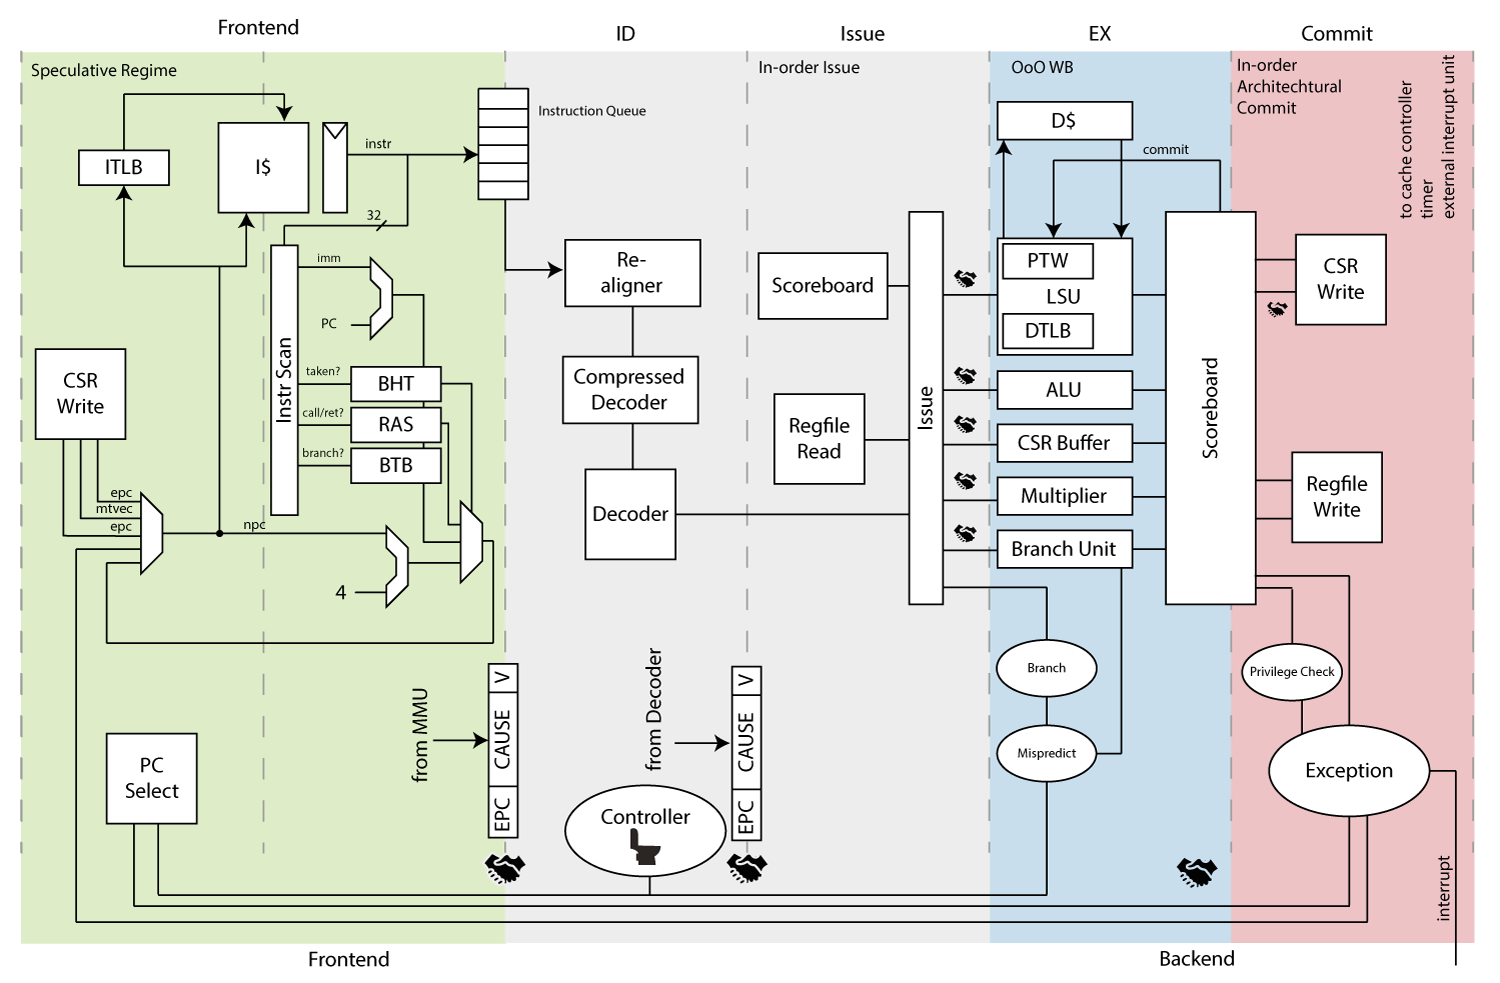
\includegraphics[width=0.7\linewidth]{cva6_design.png}
    \caption{CVA6 core design architecture.}
    \label{fig:cva6_design}
\end{figure}

The CVA6 supports any operating system based on Unix since it implements the three needed privilege levels M, S and U. The researchers wrote the core in SystemVerilog and designed its micro-architecture to reduce the critical path length. Since the developers wrote it in SystemVerilog, it is easier for someone knowledgeable in the classic Verilog and VHDL languages to understand and create a customised CPU based on the CVA6 than if they had written it in a high-level hardware description language. However, although the CVA6 is an open-source project, it is hard to take advantage of isolated hardware components. This difficulty is a consequence of how the engineers developed it. Every SystemVerilog module of the CVA6 depends on other files from the project, and the CPU itself is very little customisable. To illustrate the problem, if we wanted to remove the L1 cache present in the CVA6 to use the L1 cache used on IOb-SoC, it would be challenging and time-consuming to create a CPU core without that component.

The CVA6 can be found implemented on \textit{OpenPiton}~\cite{Balkind:2016:OOS:2872362.2872414}. \textit{OpenPiton} is an open-source project developed by the Princeton Parallel Group. With it, one can easily create an SoC that has multiple CV6 cores and run a full-feature \acrfull{os} on a development board with an FPGA.

\subsection{The Berkeley Out-of-Order \textit{RISC-V} Processor}
The Berkeley Out-of-Order \textit{RISC-V} Processor (\textit{BOOM}~\cite{zhaosonicboom}) is a superscalar \acrfull{ooo} processor executing the RV64GC variant of the \textit{RISC-V} ISA. Researchers created BOOM in the Berkeley Architecture Research group at the University of California, Berkeley. The CPU design is optimised to run on ASICs, although developers can also implement it on FPGAs. Its priority is to be a high-performance, synthesisable, and parameterisable core for architecture research. The current release, named \textit{SonicBOOM}, has one of the best performances from the publicly available open-source \textit{RISC-V} cores.

BOOM is a 10-stage CPU with the following stages: Fetch, Decode, Register Rename, Dispatch, Issue, Register Read, Execute, Memory, Writeback, and Commit. However, in most practical implementations, many of those stages are merged, generating seven stages: Fetch, Decode/Rename, Rename/Dispatch, Issue/Register Read, Execute, Memory and Writeback. Since committing happens asynchronously, it does not count as part of the \enquote{pipeline}. The BOOM developers optimised the load-store unit for the superscalar out-of-order architecture and organised the data cache into two dual-ported banks. At the front end, it is possible to customise the size of the L1 Instruction cache, the TLB, and the decode stage. Similarly to the CVA6, removing the cache from the core design and using the IOb-Cache is difficult or impossible.

This \acrshort{cpu} design is written in Chisel~\cite{bachrach2012chisel} \acrfull{hdl}. The \acrfull{chisel} allows for the production of synthesisable Verilog designs while using a high-level language to describe the hardware. \acrshort{chisel} is an adaptation of Scala~\cite{odersky2004scala} programing language, adding hardware construction primitives.

To build a \acrfull{soc} with BOOM, we would have to utilise the \textit{Rocket Chip}~\cite{asanovic2016rocket} SoC generator from CHIPS Alliance since BOOM uses micro-architecture structures (TLBs, PTWs, and others) from that tool.

\subsection{\textit{VexRiscv}}
The \textit{VexRiscv}~\cite{vexriscv} CPU is a 32-bit Linux Capable \textit{RISC-V} CPU written in the \textit{SpinalHDL}~\cite{papon2017spinalhdl}. The \textit{VexRiscv} author accomplished the hardware description of this CPU by utilising a software-oriented approach. Similarly to \acrshort{chisel}, \textit{SpinalHDL} is based on the Scala programing language.

VexRiscv is an in-order CPU with five \enquote{pipeline} stages. Many CPU plugins are optional, which add many functionalities to build a custom \textit{RISC-V} CPU. The architecture design approach in this processor is unconventional, but it has its benefits: there are remarkably few fixed hardware components; Parts of the CPU can be swapped, turned on and turned off via the plugin system; without modifying any of the CPU sources, it is possible to add new functionalities/instructions easily; It permits the CPU arrangement to cover a significantly large spectrum of implementations, allowing the construction of an entirely parametrised CPU design. When the user configures the CPU without plugins, it only includes the description of the five \enquote{pipeline} stages, their basic functionalities, and nothing else. Developers must add everything else to the CPU via plugins, including the program counter. VexRiscv can either be an application processor capable of running a full-feature \acrfull{os} or a super simple microprocessor ideal for bare-bone applications depending on how the user configures it. Contrary to \textit{BOOM}, \textit{VexRiscv} does not need any external library. Not using an external library makes it easier to generate the synthesisable Verilog file from a \textit{SpinalHDL} design.

There exists an open-source project that runs Linux with \textit{VexRiscv}, \textit{linux-on-litex-vexriscv}~\cite{litex_vexriscv}. \textit{LiteX} is used to create a \acrfull{soc} around the \textit{VexRiscv} core. \textit{LiteX} \acrshort{soc} design and peripherals are written in \textit{Migen}~\cite{bourdeauducq2012migen} another high level \acrshort{hdl}. \textit{Migen} unlike \textit{SpinalHDL} and  \acrshort{chisel} is based on Python 3.5. Because of the language describing its hardware and the way the \textit{linux-on-litex-vexriscv} project is structured, it is tough to understand how the system works, where the generated \acrshort{rtl} is and how to add custom hardware. Furthermore, \textit{linux-on-litex-vexriscv} uses \acrshort{fpga} specific hardware, making it impossible to port the system to \acrshort{asic}.

Recently the developer behind \textit{SpinalHDL} has also made public the \textit{NaxRiscv} \acrshort{cpu}. \textit{NaxRiscv} is a \acrshort{cpu} designed specifically to run a full-feature \acrlong{os}, like Linux. And just like \textit{VexRiscv}, \textit{NaxRiscv} uses \textit{SpinalHDL} to describe its hardware. Although \textit{NaxRiscv} seems like a very promising \acrshort{cpu} it is still on its early stages. Consequently, it has a primitive interface, making it complicated to implement on costume \acrfull{soc}.


\section{Overall CPU comparison}
\label{section:cpu_comparison}
In table \ref*{tab:cpu_comparison} we can see a comparison of the \acrshort{cpu}s that were presented in the previous sections, capable of running a full-feature \acrfull{os}. All of the \acrshort{cpu}s on the table are considered application processors. The reader can observe that every \acrshort{cpu} has a \acrfull{mmu}, and they all support \acrshort{user}+\acrshort{supervisor}+\acrshort{machine} privilege mode. Furthermore, all of the \acrshort{cpu}s hardware design have L1 Instruction Cache, and L1 Data cache system integrated. All \acrshort{cpu}s have an L1 cache because it makes it easier to support atomic instructions.

\textit{GNU/Linux} is the combinations of \textit{GNU} with the Linux kernel. The GNU Project developed a large part of the software comprising a complete \acrfull{os}. Many \enquote{Linux} distributions make use of that software, a few examples would be \textit{Debian}, \textit{Ubuntu}, \textit{openSUSE}, \textit{Fedora}, and the list could go on. So a processor that supports the GNU/Linux feature is a CPU capable of running a distribution like \textit{Ubuntu} or \textit{Debian}. From the table, we can see that 32-bit \textit{RISC-V} \acrshort{cpu}s are the only ones not capable of running a \textit{GNU/Linux} \acrfull{os}.

\begin{table}[!ht]
    \centering
    \resizebox{\textwidth}{!}{%
    \begin{tabular}{cccccccccc}
        & ARM                             & \multicolumn{2}{c}{Andes Technology}                      & \multicolumn{2}{c}{SiFive}                                & PULP platform                 & UC Berkeley                 & \multicolumn{2}{c}{SpinalHDL}                                 \\ \cline{2-10}
\multicolumn{1}{c|}{}                                                                   & \multicolumn{1}{c|}{Cortex-A72} & \multicolumn{1}{c|}{A25}    & \multicolumn{1}{c|}{AX25}   & \multicolumn{1}{c|}{U54}    & \multicolumn{1}{c|}{U74}    & \multicolumn{1}{c|}{CVA6}      & \multicolumn{1}{c|}{BOOM}   & \multicolumn{1}{c|}{VexRiscv} & \multicolumn{1}{c|}{NaxRiscv} \\ \hline
\multicolumn{1}{|c|}{\begin{tabular}[c]{@{}c@{}}Architecture\\ bit widths\end{tabular}} & \multicolumn{1}{c|}{64-bit}     & \multicolumn{1}{c|}{32-bit} & \multicolumn{1}{c|}{64-bit} & \multicolumn{1}{c|}{64-bit} & \multicolumn{1}{c|}{64-bit} & \multicolumn{1}{c|}{32/64-bit} & \multicolumn{1}{c|}{64-bit} & \multicolumn{1}{c|}{32-bit}   & \multicolumn{1}{c|}{64-bit}   \\ \hline
\multicolumn{1}{|c|}{MMU}                                                               & \multicolumn{1}{c|}{Y}          & \multicolumn{1}{c|}{Y}      & \multicolumn{1}{c|}{Y}      & \multicolumn{1}{c|}{Y}      & \multicolumn{1}{c|}{Y}      & \multicolumn{1}{c|}{Y}         & \multicolumn{1}{c|}{Y}      & \multicolumn{1}{c|}{Y}        & \multicolumn{1}{c|}{Y}        \\ \hline
\multicolumn{1}{|c|}{FPU}                                                               & \multicolumn{1}{c|}{Y}          & \multicolumn{1}{c|}{Y}      & \multicolumn{1}{c|}{Y}      & \multicolumn{1}{c|}{Y}      & \multicolumn{1}{c|}{Y}      & \multicolumn{1}{c|}{X}         & \multicolumn{1}{c|}{Y}      & \multicolumn{1}{c|}{Y}        & \multicolumn{1}{c|}{Y}        \\ \hline
\multicolumn{1}{|c|}{\begin{tabular}[c]{@{}c@{}}16-bit \\ instructions\end{tabular}}    & \multicolumn{1}{c|}{X}          & \multicolumn{1}{c|}{Y}      & \multicolumn{1}{c|}{Y}      & \multicolumn{1}{c|}{Y}      & \multicolumn{1}{c|}{Y}      & \multicolumn{1}{c|}{Y}         & \multicolumn{1}{c|}{Y}      & \multicolumn{1}{c|}{Y}        & \multicolumn{1}{c|}{X}        \\ \hline
\multicolumn{1}{|c|}{Cache L1(I+D)}                                                     & \multicolumn{1}{c|}{Y}          & \multicolumn{1}{c|}{Y}      & \multicolumn{1}{c|}{Y}      & \multicolumn{1}{c|}{Y}      & \multicolumn{1}{c|}{Y}      & \multicolumn{1}{c|}{Y}         & \multicolumn{1}{c|}{Y}      & \multicolumn{1}{c|}{Y}        & \multicolumn{1}{c|}{Y}        \\ \hline
\multicolumn{1}{|c|}{\begin{tabular}[c]{@{}c@{}}Interrupt \\ Controller\end{tabular}}   & \multicolumn{1}{c|}{X}          & \multicolumn{1}{c|}{Y}      & \multicolumn{1}{c|}{Y}      & \multicolumn{1}{c|}{Y}      & \multicolumn{1}{c|}{Y}      & \multicolumn{1}{c|}{X}         & \multicolumn{1}{c|}{X}      & \multicolumn{1}{c|}{X}        & \multicolumn{1}{c|}{X}        \\ \hline
\multicolumn{1}{|c|}{\acrshort{user}+\acrshort{supervisor}+\acrshort{machine} Mode}                                                        & \multicolumn{1}{c|}{N/A}        & \multicolumn{1}{c|}{Y}      & \multicolumn{1}{c|}{Y}      & \multicolumn{1}{c|}{Y}      & \multicolumn{1}{c|}{Y}      & \multicolumn{1}{c|}{Y}         & \multicolumn{1}{c|}{Y}      & \multicolumn{1}{c|}{Y}        & \multicolumn{1}{c|}{Y}        \\ \hline
\multicolumn{1}{|c|}{GNU/Linux}                                                         & \multicolumn{1}{c|}{Y}          & \multicolumn{1}{c|}{X}      & \multicolumn{1}{c|}{Y}      & \multicolumn{1}{c|}{Y}      & \multicolumn{1}{c|}{Y}      & \multicolumn{1}{c|}{Y}         & \multicolumn{1}{c|}{Y}      & \multicolumn{1}{c|}{X}        & \multicolumn{1}{c|}{Y}        \\ \hline
\multicolumn{1}{|c|}{Open-Source}                                                       & \multicolumn{1}{c|}{X}          & \multicolumn{1}{c|}{X}      & \multicolumn{1}{c|}{X}      & \multicolumn{1}{c|}{X}      & \multicolumn{1}{c|}{X}      & \multicolumn{1}{c|}{Y}         & \multicolumn{1}{c|}{Y}      & \multicolumn{1}{c|}{Y}        & \multicolumn{1}{c|}{Y}        \\ \hline
\end{tabular}%
    }
    \caption{CPU comparison table: Y means the CPU supports the feature; X means the CPU does not support the feature; N/A means the feature does not apply to the respective CPU.}
    \label{tab:cpu_comparison}
\end{table}
